% main.tex — entry point for the thesis (SNU IE kor-ms format)
%
% BUILD (from thesis/):
%   latexmk -pdf main.tex
%
% ============================================================================
% DOCUMENT SCHEME
% ============================================================================
%
%  FRONT MATTER (Roman / roman page numbers)
%  ├── makefrontcover                  Undergraduate cover page
%  ├── abstract.tex                    Korean abstract (초록)
%  └── contents.tex                    목차, 표 목차, 그림 목차
%
%  BODY (arabic page numbers)
%  ├── 01_introduction … 05_conclusion
%  └── appendix/
%
%  BACK MATTER
%  ├── references.bib      Inside bibpage environment
%  ├── abstract_en.tex     English abstract
%  └── acknowledgments.tex 감사의 글
%
% ============================================================================

% Shared preamble — SNU IE department thesis format (kor-ms).
%
% BUILD (from thesis/):
%   latexmk -pdf main.tex

\RequirePackage{fix-cm}

\documentclass[oneside, ko, ms]{snuthesis_utf8_kor}

%%%%%%%%%%%%%%%%%%%%%%%%%%%%%%%%%%%%%%%%
%% Table of contents (Korean labels)
%%%%%%%%%%%%%%%%%%%%%%%%%%%%%%%%%%%%%%%%
\usepackage[titles]{tocloft}
\usepackage{amsmath,amssymb,amsthm,kotex,color}
\usepackage{graphicx}
\usepackage{tikz}
\usetikzlibrary{shapes,arrows}
\usepackage{algpseudocode,algorithm,algorithmicx}
\usepackage{setspace}
\usepackage{array}
\usepackage{romanbar}
\usepackage{pgfplots}
\usepackage{caption}
\usepackage{subcaption}
\usepackage{booktabs,multirow}
\usepackage{threeparttable}
\usepackage{rotating}
\usepackage{comment}
\usepackage[numbers,sort&compress]{natbib}

\pgfplotsset{compat=1.18}

\makeatletter
\renewcommand\cftchappresnum{제 ~}
\renewcommand\cftchapaftersnum{ ~ 장}
\renewcommand\cftfigpresnum{그림 ~}
\renewcommand\cfttabpresnum{표 ~}
\renewcommand{\algorithmicforall}{\textbf{foreach}}

\newtheorem{theorem}{Theorem}[chapter]
\newtheorem{lemma}[theorem]{Lemma}
\newtheorem{proposition}[theorem]{Proposition}
\newtheorem{corollary}[theorem]{Corollary}
\newtheorem{definition}[theorem]{Definition}
\newtheorem{Proposition}{Proposition}
\newtheorem{remark}{Remark}[chapter]
\newtheorem{example}{Example}[chapter]

\usepackage[pdftex,bookmarks=true]{hyperref}
\hypersetup{
  colorlinks=true,
  linkcolor=black,
  citecolor=blue,
  urlcolor=blue,
}
\usepackage{cleveref}

\makeatother

\newlength{\mytmplen}
\settowidth{\mytmplen}{\bfseries\cftchappresnum\cftchapaftersnum}
\addtolength{\cftchapnumwidth}{\mytmplen}
\settowidth{\mytmplen}{\bfseries\cftfigpresnum\cftfigaftersnum}
\addtolength{\cftfignumwidth}{\mytmplen}
\settowidth{\mytmplen}{\bfseries\cfttabpresnum\cfttabaftersnum}
\addtolength{\cfttabnumwidth}{\mytmplen}

%%%%%%%%%%%%%%%%%%%%%%%%%%%%%%%%%%%%%%%%
%% Thesis metadata — fill in before submission
%%%%%%%%%%%%%%%%%%%%%%%%%%%%%%%%%%%%%%%%
\title{조합 최적화를 위한 확산 모델}
\title*{Diffusion Models for Combinatorial Optimization}
\titlen{Diffusion Models for Combinatorial Optimization}

\author{Janghyeok Choi}
\author*{최장혁}
\authorn{최~장~혁}
\phonenumber{010-0000-0000}
\studentnumber{2020-12053}

\advisor{지도교수 성함}        % Korean name on approval page
\advisor*{Advisor Name}        % English name (optional)
\advisorn{지~도~교~수}          % Spaced Korean name for approval page

\graddate{2026~년~~2~월}
\submissiondate{2026~년~~1~월}
\submissiondaten{2026~년~~1~월~~15~일}
\approvaldate{2026~년~~2~월}

\committeemembers%
{위원장 성함}%
{지도교수 성함}%
{위원 성함}%
{}%
{}%

\setlength{\committeenameunderlinelength}{5cm}


\begin{document}

\pagenumbering{Roman}
\makefrontcover

\cleardoublepage
\pagenumbering{roman}

\keyword{조합최적화, 확산모델, 강화학습, 신경망 조합최적화, 차량 경로 문제}
\begin{abstract}
본 논문에서는 조합 최적화 문제를 확산 기반 신경망 해법으로 다룬다.
확산 모델이 생성하는 열지도(heatmap)를 문제 제약을 만족하는 해로 디코딩하는 과정이
성능의 핵심 병목이며, 이를 완화하기 위해 CADO 스타일의 디코더 인식 강화학습
미세조정을 적용한다.
TSP, CVRP, MDVRP에 대한 실험을 통해 제안 방법의 최적성 간격(gap), 계산 비용,
및 주요 절제(ablation) 결과를 보고한다.
\end{abstract}

\tableofcontents
\addcontentsline{toc}{chapter}{\contentsname}
\cleardoublepage

\listoftables
\addcontentsline{toc}{chapter}{\listtablename}
\cleardoublepage

\listoffigures
\addcontentsline{toc}{chapter}{\listfigurename}
\cleardoublepage


\cleardoublepage
\pagenumbering{arabic}

\chapter{Introduction}
\label{ch:introduction}

\section{Motivation}
\label{sec:motivation}
% NP-hard routing problems; limits of classical solvers vs. learned heuristics.

\section{Problem Statement}
\label{sec:problem-statement}
% TSP and CVRP (optionally MDVRP); objective (tour cost / gap to optimum).

\section{Contributions}
\label{sec:contributions}
\begin{itemize}
  \item Reproduce and extend \emph{DifusCO}-style diffusion solvers for TSP and CVRP.
  \item Implement \emph{CADO}-style hybrid fine-tuning and REINFORCE on top of supervised checkpoints.
  \item Empirical comparison: optimality gap, wall-clock cost, and ablations (reward mode, entropy, denoising steps).
\end{itemize}

\section{Thesis Outline}
\label{sec:outline}
% Brief pointer to each following chapter (one sentence each).

\chapter{Literature Review}
\label{ch:Literature Review}

\section{Optimization Problems}
\label{sec:optimization-problems}

\subsection{Combinatorial Optimization}
\label{subsec:combinatorial-optimization}

This paper follows the conventional notation for combinatorial optimization introduced by
\citet{papadimitriou1998combinatorial}. The space of candidate solutions for a CO problem
instance $s$ is denoted by $\mathcal{X}_s = \{0, 1\}^N$, and the objective function is denoted
by $c_s: \mathcal{X}_s \rightarrow \mathbb{R}$ for a solution $x \in \mathcal{X}_s$.
Given a cost function $c_s(\cdot)$, the goal is to find the optimal solution $x^{s*}$ for
the given instance $s$:
\[
x^{s*} = \arg\min_{x \in \mathcal{X}_s} c_s(x).
\]

Because enumerating all possible solution sets for a CO problem is computationally
intractable, exact methods often relax the binary condition, solve a linear program (LP), and
subsequently branch on fractional solution components. This approach is known as branch and
bound (B\&B). While B\&B avoids enumerating entirely unnecessary solution sets, the number of
branches can still grow exponentially in the worst case.

\subsection{Traveling Salesman Problem}
\label{subsec:tsp}

Let $G = (V, E)$ be a complete undirected graph with $|V| = n$ cities and edge costs
$c_{ij} \ge 0$ for all $\{i,j\} \in E$. Define binary decision variables
\[
x_{ij} =
\begin{cases}
1, & \text{if the tour uses edge } \{i,j\},\\
0, & \text{otherwise.}
\end{cases}
\]

The traveling salesman problem (TSP) can be formulated as the following integer program:
\[
\begin{aligned}
\min_{x}\quad & \sum_{\{i,j\}\in E} c_{ij} x_{ij} \\
\text{s.t.}\quad
& \sum_{j\in V\setminus\{i\}} x_{ij} = 2, && \forall i\in V
  \quad \text{(degree constraints)}\\
& \sum_{\{i,j\}\in E(S)} x_{ij} \le |S|-1, && \forall S\subset V,\; 2\le |S|\le n-1
  \quad \text{(subtour elimination)}\\
& x_{ij}\in\{0,1\}, && \forall \{i,j\}\in E.
\end{aligned}
\]
Here, $E(S) = \{\{i,j\}\in E : i\in S,\; j\in S\}$ denotes the set of edges with both
endpoints in subset $S$. The subtour elimination constraints enforce that the selected edges
form a single Hamiltonian cycle visiting every city exactly once, rather than multiple
disjoint cycles.

\subsection{Capacitated Vehicle Routing Problem}
\label{subsec:cvrp}

Let $G=(V,E)$ be a complete graph where $V = \{0,1,\dots,n\}$, with depot $0$ and customers
$1,\dots,n$. Each customer $i\in\{1,\dots,n\}$ has demand $q_i>0$, and $c_{ij}\ge 0$ is the
travel cost between nodes $i$ and $j$. A fleet of at most $m$ identical vehicles is available,
each with capacity $Q$. Define binary decision variables
\[
x_{ij}=
\begin{cases}
1, & \text{if a vehicle travels directly from } i \text{ to } j,\\
0, & \text{otherwise,}
\end{cases}
\qquad \forall i\ne j,\; i,j\in V,
\]
and continuous load variables $u_i$ for $i\in\{1,\dots,n\}$ denoting the cumulative load
delivered upon arrival at customer $i$.

The capacitated vehicle routing problem (CVRP) can be formulated as the following
mixed-integer program:
\[
\begin{aligned}
\min_{x,u}\quad & \sum_{i\in V}\sum_{j\in V\setminus\{i\}} c_{ij}x_{ij}\\
\text{s.t.}\quad
& \sum_{j\in V\setminus\{i\}} x_{ij} = 1, && \forall i\in V\setminus\{0\}
  \quad \text{(each customer departs once)}\\
& \sum_{i\in V\setminus\{j\}} x_{ij} = 1, && \forall j\in V\setminus\{0\}
  \quad \text{(each customer arrives once)}\\
& \sum_{j\in V\setminus\{0\}} x_{0j} \le m, && \text{(number of routes)}\\
& \sum_{i\in V\setminus\{0\}} x_{i0}
  = \sum_{j\in V\setminus\{0\}} x_{0j}, && \text{(flow conservation at depot)}\\
& q_i \le u_i \le Q, && \forall i\in V\setminus\{0\}
  \quad \text{(capacity bounds)}\\
& u_i - u_j + Qx_{ij} \le Q - q_j, &&
  \forall i,j\in V\setminus\{0\},\; i\ne j
  \quad \text{(MTZ)}\\
& x_{ij}\in\{0,1\}, && \forall i\ne j,\; i,j\in V.
\end{aligned}
\]
The Miller--Tucker--Zemlin (MTZ) constraints enforce route connectivity and eliminate
subtours while simultaneously ensuring that vehicle capacity is not exceeded.

\subsection{Multi-Depot Vehicle Routing Problem}
\label{subsec:mdvrp}

Let $G=(V,E)$ be a complete graph containing multiple depots and customers. Let
$D=\{0,1,\dots,d\}$ be the set of depots and $C=\{d+1,\dots,d+n\}$ the set of customers, such
that $V=D\cup C$ and $D\cap C=\emptyset$. Depot $k\in D$ has at most $m_k$ identical vehicles
available, and each customer $i\in C$ has demand $q_i>0$. Let $c_{ij}\ge 0$ denote the travel
cost between nodes $i$ and $j$, and let $V_k=C\cup\{k\}$ be the customer set together with
depot $k$. Define depot-indexed binary decision variables
\[
x_{ij}^k=
\begin{cases}
1, & \text{if a vehicle from depot } k \text{ travels directly from } i \text{ to } j,\\
0, & \text{otherwise,}
\end{cases}
\qquad \forall k\in D,\; i\ne j,\; i,j\in V_k,
\]
and assignment variables
\[
y_{ik}=
\begin{cases}
1, & \text{if customer } i \text{ is served by depot } k,\\
0, & \text{otherwise,}
\end{cases}
\qquad \forall i\in C,\; k\in D.
\]

The multi-depot vehicle routing problem (MDVRP) can be formulated as the following
mixed-integer program:
\[
\begin{aligned}
\min_{x,y}\quad
& \sum_{k\in D}\sum_{i\in V_k}\sum_{j\in V_k\setminus\{i\}} c_{ij}x_{ij}^k\\
\text{s.t.}\quad
& \sum_{k\in D} y_{ik} = 1, && \forall i\in C
  \quad \text{(assign each customer to one depot)}\\
& \sum_{j\in V_k\setminus\{i\}} x_{ij}^k = y_{ik}, &&
  \forall i\in C,\; \forall k\in D
  \quad \text{(customer departure)}\\
& \sum_{j\in V_k\setminus\{i\}} x_{ji}^k = y_{ik}, &&
  \forall i\in C,\; \forall k\in D
  \quad \text{(customer arrival)}\\
& \sum_{j\in C} x_{kj}^k = \sum_{j\in C} x_{jk}^k \le m_k, && \forall k\in D
  \quad \text{(depot flow and route count)}\\
& \sum_{i\in S}\sum_{j\in S\setminus\{i\}} x_{ij}^k \le |S|-1, &&
  \forall k\in D,\; \forall S\subseteq C,\; 2\le |S|\le n-1
  \quad \text{(subtour elimination)}\\
& x_{ij}^k\in\{0,1\}, && \forall k\in D,\; i\ne j,\; i,j\in V_k,\\
& y_{ik}\in\{0,1\}, && \forall i\in C,\; k\in D.
\end{aligned}
\]
If vehicle capacities are included, standard capacity constraints, such as MTZ- or flow-based
constraints within each depot's routes, can be added to ensure that the total demand on any
route does not exceed the vehicle capacity.

\section{Classical and Learning-Based Solvers}
\label{sec:solvers}

Combinatorial optimization solvers can be broadly grouped into exact methods,
relaxation-based methods, and heuristic or metaheuristic methods. In practice, modern
state-of-the-art solvers frequently combine these ideas.

\subsection{Exact Solvers}
\label{subsec:exact-solvers}

Exact solvers provide guaranteed optimality, but their computational cost can grow
exponentially. Branch and bound (B\&B) builds a search tree over partial solutions. At each
node, it computes a lower bound, typically through a relaxation such as an LP relaxation. If
the bound is worse than the best-known feasible solution, which acts as an upper bound, the
node is pruned. B\&B is exact, but the search tree can still become exponentially large.

Branch and cut (B\&C) augments B\&B with cutting planes. When the LP relaxation yields a
fractional solution, the solver adds valid inequalities, or cuts, that remove the fractional
solution while preserving all integer-feasible solutions. For the TSP, subtour elimination
constraints serve as classic cuts. This strategy forms the backbone of solvers such as
Concorde \citep{applegate2006traveling}.

Branch and price (B\&P) combines B\&B with column generation. Instead of enumerating all
variables, which is often exponential, the solver optimizes a restricted master problem and
repeatedly generates new variables by solving a pricing subproblem. VRP formulations that use
route variables commonly employ this approach.

\subsection{Relaxation and Decomposition Methods}
\label{subsec:relaxation-decomposition}

Relaxation and decomposition methods are widely used to obtain bounds and exploit scalable
problem structure. LP relaxation replaces integrality constraints with continuous constraints
such as $x \in [0,1]$, yielding a linear program. LP relaxations provide lower bounds and are
standard components in B\&B and B\&C frameworks, although their fractional solutions may differ
substantially from integer-feasible solutions.

Lagrangian relaxation moves hard constraints into the objective function using multipliers.
This transformation can produce decomposable subproblems and often yields strong bounds,
especially for routing and scheduling problems. Benders decomposition instead splits variables
into a master problem and a subproblem. The subproblem generates Benders cuts that iteratively
refine the master problem, making the approach effective for problems with naturally separable
structure.

\subsection{Heuristics and Metaheuristics}
\label{subsec:heuristics-metaheuristics}

Heuristics and metaheuristics are designed to obtain high-quality feasible solutions quickly.
Local search iteratively improves a feasible solution through small neighborhood moves. In
routing problems, common operations include 2-opt, 3-opt, relocate, swap, and cross-exchange.
Although local search is fast and effective, it is susceptible to local minima.

Metaheuristics are higher-level strategies designed to escape local minima or explore the
solution space more broadly. Prominent examples include simulated annealing (SA), which
occasionally accepts worse moves according to a temperature schedule; tabu search, which uses
memory to avoid cycling back to recently visited solutions; genetic algorithms (GA), which
maintain a population of solutions through crossover and mutation; and ant colony optimization
(ACO), which constructs solutions probabilistically based on pheromone trails. These methods
do not guarantee optimality but are highly competitive for large instances.

\subsection{Learning-Assisted Solvers}
\label{subsec:learning-assisted-solvers}

Recent neural CO research often integrates traditional solvers in two distinct roles. First,
exact or high-quality heuristic solutions can serve as teachers or oracles, providing
ground-truth labels for supervised learning. Second, classical methods can act as decoding or
refinement steps: neural models generate a soft solution, such as a probabilistic heatmap,
which is subsequently transformed into a feasible hard solution using greedy decoding, local
search such as 2-opt, or other solver components.

In summary, exact solvers provide optimality guarantees at high computational cost,
relaxations and decompositions offer scalable bounds, and heuristics provide strong solutions
rapidly. Modern NCO systems frequently combine all three, aiming to address the limitations of
traditional solvers through data-driven advantages.

\section{Neural Network Methodologies}
\label{sec:neural-network-methodologies}

\subsection{Graph Neural Networks}
\label{subsec:gnn}

Graph neural networks (GNNs) are neural architectures designed to process data defined on
graphs by repeatedly performing message passing. Each node updates its representation by
aggregating transformed features from its neighbors. In each layer, a generic GNN computes
\[
h_i^{\ell+1}=\phi\Big(h_i^{\ell},\;
\operatorname{AGG}_{j\in\mathcal{N}(i)}\psi(h_i^{\ell},h_j^{\ell},e_{ij})\Big),
\]
where $h_i^{\ell}$ is the node embedding at layer $\ell$, $e_{ij}$ is an optional edge
feature, and $\operatorname{AGG}$ is a permutation-invariant operator such as summation or
mean aggregation.

In neural combinatorial optimization, classical backbones such as graph convolutional
networks (GCNs) \citep{kipf2016semi} and graph attention networks (GATs)
\citep{velickovic2017graph} primarily produce node embeddings. This is sufficient when the
target variable is node-based, such as predicting whether a node is selected in the maximum
independent set (MIS). However, for routing problems such as the TSP, the key latent variable
is often edge-based, indicating whether an edge belongs to the tour. Consequently, a standard
node-centric GNN requires additional structural mechanisms to reliably represent and predict
edge decisions.

\subsection{Anisotropic Graph Neural Networks}
\label{subsec:agnn}

Anisotropic graph neural networks (AGNNs) extend traditional message passing by maintaining
both node and edge embeddings and by using edge gates so that information flow depends on the
current edge state. This architecture is especially useful for diffusion-style denoising
networks, where the model ingests noisy variables $x_t$, such as node states for MIS or edge
states for TSP, and predicts the clean variables $x_0$.

Let $h_i^{\ell}$ and $e_{ij}^{\ell}$ denote node and edge features at layer $\ell$, and let
$t$ be a sinusoidal timestep embedding. A standard AGNN layer used in diffusion backbones
first performs an anisotropic edge update:
\[
\hat{e}_{ij}^{\ell+1}=P^{\ell}e_{ij}^{\ell}+Q^{\ell}h_i^{\ell}+R^{\ell}h_j^{\ell}.
\]
The edges are then refined with residual multilayer perceptrons (MLPs) and timestep
conditioning:
\[
e_{ij}^{\ell+1}
=e_{ij}^{\ell}+\operatorname{MLP}_e(\operatorname{BN}(\hat{e}_{ij}^{\ell+1}))
+\operatorname{MLP}_t(t).
\]

The node update then uses edge-gated messages:
\[
h_i^{\ell+1}=h_i^{\ell}+\alpha\Big(
\operatorname{BN}\big(U^{\ell}h_i^{\ell}
+\sum_{j\in\mathcal{N}(i)}
\sigma(\hat{e}_{ij}^{\ell+1})\odot V^{\ell}h_j^{\ell}\big)\Big).
\]
Here $\sigma(\cdot)$ is a sigmoid gate and $\odot$ is the Hadamard product. Intuitively, each
neighbor's message is filtered by the current edge embedding, allowing the network to
emphasize or suppress interactions in a direction- and edge-dependent manner.

Because AGNNs jointly model nodes and edges, they naturally support optimization tasks that
require edge-variable prediction, such as the TSP. For these problems, $e_{ij}^{0}$ is
initialized from the noisy edge variables $x_t$, and $h_i^{0}$ is set to positional or
sinusoidal node features. The final network head then predicts denoised edge probabilities or
values.

\section{Diffusion Models for COP}
\label{sec:diffusion-cop}

\subsection{DIFUSCO}
\label{subsec:difusco}

DIFUSCO (Diffusion for Combinatorial Optimization) solves CO problems by casting a feasible
solution as a binary structure, learning a diffusion-style denoising process to transform
random noise into that structure, and finally applying a classical decoder, such as greedy
decoding followed by 2-opt, to yield a valid tour or route \citep{sun2023difusco}.

\subsubsection{Representation}
\label{subsec:difusco-representation}

DIFUSCO represents the target solution as a binary variable $x_0\in\{0,1\}^N$. For TSP,
$x_0$ typically corresponds to edge decisions, indicating whether an edge is included in the
tour. Thus, $N$ scales with the number of candidate edges.

\subsubsection{Forward Process}
\label{subsec:difusco-forward}

A Markov chain gradually corrupts the optimal solution $x_0$ into random noise $x_T$ using a
variance schedule $\{\beta_t\}_{t=1}^T$. In discrete diffusion, the solution $x$ is converted
to a one-hot representation $\tilde{x}\in\{0,1\}^{N\times 2}$ and subjected to a categorical
transition:
\[
q(x_t\mid x_{t-1}) = \mathrm{Cat}(x_t;\,p=\tilde{x}_{t-1}Q_t),\quad
Q_t=\begin{pmatrix}
1-\beta_t & \beta_t\\
\beta_t & 1-\beta_t
\end{pmatrix}.
\]
As $\prod_{t=1}^T(1-\beta_t)\approx 0$, the terminal distribution becomes near-uniform.

For continuous diffusion on discrete data, the discrete solution $x_0\in\{0,1\}^N$ is
rescaled to $\hat{x}_0\in\{-1,1\}^N$ and subjected to Gaussian corruption:
\[
q(\hat{x}_t\mid \hat{x}_{t-1})
:= \mathcal{N}(\hat{x}_t;\sqrt{1-\beta_t}\,\hat{x}_{t-1},\,\beta_t I).
\]
This ensures that $\hat{x}_T$ approaches a standard Gaussian distribution when
$\prod_{t=1}^T(1-\beta_t)\approx 0$.

\subsubsection{Reverse Process}
\label{subsec:difusco-reverse}

DIFUSCO learns the reverse transitions defined by
\[
p_\theta(x_0) := \int p_\theta(x_{0:T})\,dx_{1:T},\quad
p_\theta(x_{0:T}) = p(x_T)\prod_{t=1}^T p_\theta(x_{t-1}\mid x_t).
\]
This is achieved by optimizing the standard variational lower bound, which yields
Kullback--Leibler (KL) divergence terms of the form
\[
D_{\mathrm{KL}}\big(q(x_{t-1}\mid x_t,x_0)\,\|\,p_\theta(x_{t-1}\mid x_t)\big).
\]

The neural network prediction target depends on the diffusion type. In discrete diffusion,
the denoiser is trained to predict the clean variable $p_\theta(x_0\mid x_t)$. The reverse
step is formed by substituting the prediction into the true posterior:
\[
p_\theta(x_{t-1}\mid x_t) \approx q(x_{t-1}\mid x_t,\hat{x}_0),\quad
\hat{x}_0\sim p_\theta(x_0\mid x_t).
\]
In continuous diffusion, the denoiser predicts the Gaussian noise $\varepsilon_t$:
\[
\varepsilon_t
= \frac{\hat{x}_t-\sqrt{\bar{\alpha}_t}\,\hat{x}_0}
{\sqrt{1-\bar{\alpha}_t}}
= f_\theta(\hat{x}_t,t),
\]
which is used to formulate a point estimate of $\hat{x}_0$ inside the Gaussian posterior for
$\hat{x}_{t-1}$.

\subsubsection{AGNN Denoiser}
\label{subsec:difusco-agnn-denoiser}

The conditional model $f_\theta(\cdot,t)$ is implemented using an edge-aware AGNN backbone
with timestep conditioning. After sampling the denoised representation to obtain a continuous
or probabilistic $x_0$, the model applies thresholding or quantization to map the heatmap back
to the $\{0,1\}$ domain. Finally, a non-differentiable decoder, such as greedy edge selection,
and optional local improvement heuristics, such as 2-opt, are applied to enforce hard
feasibility constraints and minimize the final objective value.

\section{Reinforcement Learning Fine-Tuning}
\label{sec:rl-ft}

\subsection{CADO}
\label{subsec:cado}

While diffusion-based models such as DIFUSCO demonstrate strong performance using supervised
learning (SL), this paradigm suffers from a fundamental objective mismatch. In SL, the neural
network is trained to imitate optimal ground-truth solutions by minimizing surrogate losses,
such as cross-entropy. However, minimizing this imitation loss does not guarantee minimizing
the actual decoded solution cost.

CADO (Cost-Aware Diffusion Solvers for Combinatorial Optimization through RL Fine-Tuning)
analyzes this objective mismatch through two main deficiencies \citep{yoon2024cado}. The
first is decoder-blindness: the SL objective is oblivious to the non-differentiable decoding
heuristic $f_g$, such as greedy search or 2-opt, that projects the continuous heatmap into a
discrete feasible solution. The second is cost-blindness: SL prioritizes structural similarity
to the ground-truth solution over the actual objective value of the problem. Empirical results
in CADO show that structural proximity to an optimal solution, measured by Hamming distance,
can have near-zero correlation with the final decoded solution cost.

To address these issues, CADO introduces a reinforcement learning (RL) fine-tuning framework
that explicitly aligns the diffusion process with the true CO objective.

\subsection{MDP Formulation}
\label{subsec:cado-mdp}

Instead of relying only on structural imitation, CADO directly optimizes the post-decoded
solution cost by formulating the iterative diffusion denoising process as a Markov decision
process (MDP). This formulation enables the model to be trained using the REINFORCE
algorithm.

Let the MDP be represented by the tuple $(\mathcal{S}, \mathcal{A}, P, \rho_0, R)$. The
state $s_t\in\mathcal{S}$, action $a_t\in\mathcal{A}$, and reward function $R(s_t,a_t)$ at
timestep $t$ are defined as
\[
s_t \triangleq (g, T-t, x_{T-t}), \quad a_t \triangleq x_{t-1},
\]
and
\[
R(s_t, a_t) \triangleq
\begin{cases}
-c_g(f_g(x_0)), & \text{if } t = T, \\
0, & \text{otherwise.}
\end{cases}
\]
Here, $g$ represents the problem instance, $c_g(\cdot)$ is the true cost function, and
$f_g(\cdot)$ is the non-differentiable decoder. By evaluating the reward only at the final
step, after the heatmap has been fully decoded, this formulation explicitly incorporates both
the decoder's behavior and the true cost feedback, resolving decoder-blindness and
cost-blindness.

\subsection{Reward Strategies}
\label{subsec:cado-reward-strategies}

To stabilize RL training and reduce variance, CADO uses two reward formulation strategies.
The standard reward (SR) uses the negative true solution cost directly as the reward signal.
This label-free formulation enables the model to learn through trial-and-error exploration and
can remain applicable even when labeled solutions are unavailable.

The label-centered reward (LCR) uses information from the SL pre-training dataset without
returning to pure imitation. It repurposes the ground-truth solution cost $b_D(g)$ as an
instance-specific baseline and defines the reward as the negative optimality gap:
\[
R_t = -\big(c_g(f_g(x_0)) - b_D(g)\big).
\]
Because the baseline $b_D(g)$ depends only on the problem instance and is independent of the
policy's actions, it serves as an unbiased baseline. Thus, the policy gradient remains
consistent with true cost minimization even if the dataset labels are computationally
suboptimal.

\subsection{Hybrid Fine-Tuning}
\label{subsec:cado-hybrid-ft}

Applying RL fine-tuning naively to the large AGNN architectures used in diffusion models can
be unstable and memory-intensive. To achieve parameter-efficient and stable adaptation, CADO
employs a hybrid fine-tuning (Hybrid-FT) strategy.

Hybrid-FT applies low-rank adaptation (LoRA) to the input layer and most backbone GNN layers.
This preserves the robust features learned during SL pre-training while introducing only a
small set of trainable low-rank matrices. At the same time, CADO applies selective layer
fine-tuning (Selective-FT), in which all parameters are retrained, to the final GNN layer and
the output layer. These layers are most directly responsible for final heatmap generation. The
combination supports rapid initial convergence while maintaining sufficient expressive power
for cost-aware adaptation.


\chapter{Methodology}
\label{ch:methodology}

\section{Overview}
\label{sec:method-overview}

This thesis develops and evaluates diffusion-based neural solvers for routing problems. The proposed methodology follows a two-stage training pipeline. First, a DIFUSCO-style graph diffusion model is trained with supervised denoising using solver-generated reference solutions \citep{sun2023difusco}. Second, the supervised checkpoint can be further adapted using a CADO-style reinforcement learning objective that directly rewards the quality of the decoded solution \citep{yoon2024cado}.

The motivation for this design is that supervised denoising provides stable training for high-dimensional binary solution structures, while reinforcement learning fine-tuning reduces the mismatch between the training objective and the final evaluation objective. In supervised learning, the model is trained to imitate reference binary labels. However, routing performance is ultimately determined only after the predicted heatmap is passed through a non-differentiable decoder. Therefore, the second stage explicitly incorporates the decoder and the decoded solution cost into the training signal.

\begin{figure}[htbp]
    \centering
    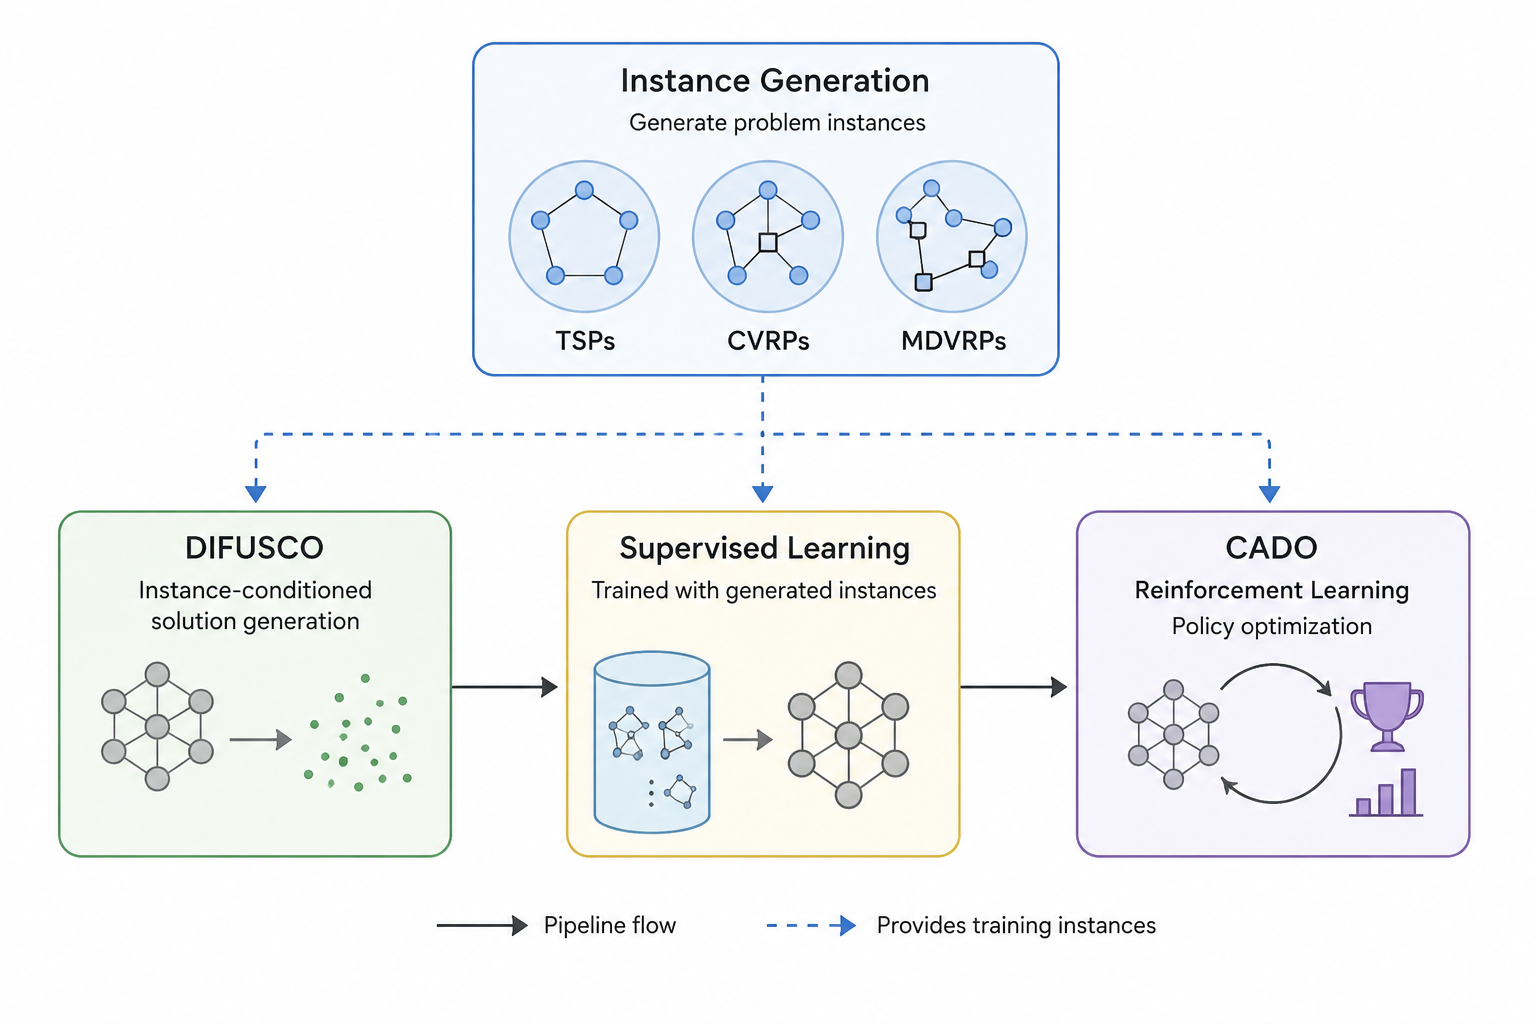
\includegraphics[width=0.85\textwidth]{./figures/pipeline.png}
    \caption{
        Overview of the proposed training and evaluation pipeline. A DIFUSCO-style diffusion model is first trained by supervised denoising on solver-generated binary labels \citep{sun2023difusco}. The trained checkpoint can then be fine-tuned with a CADO-style reinforcement learning objective based on decoded solution quality \citep{yoon2024cado}.
    }
    \label{fig:pipeline}
\end{figure}

The implementation covers three routing settings: the Traveling Salesman Problem (TSP), the Capacitated Vehicle Routing Problem (CVRP), and the Multi-Depot Vehicle Routing Problem (MDVRP). For TSP, the model predicts a heatmap over candidate tour edges. For CVRP, the same edge-heatmap formulation is extended to multi-route vehicle routing by adding depot and demand information to the node representation and by enforcing capacity during decoding. For MDVRP, this thesis considers an assignment-level formulation in which the model predicts customer--depot assignment scores. Therefore, TSP and CVRP are evaluated using decoded route cost and relative gap to a reference solution, whereas MDVRP is evaluated using assignment-level metrics such as depot-assignment accuracy and capacity-violation rate.

\section{Binary Solution Representation}
\label{sec:binary-solution-representation}

Following the graph-based diffusion formulation of DIFUSCO \citep{sun2023difusco}, each optimization instance is represented by a binary solution vector. Let \(s\) denote a problem instance and let
\[
    x_0 \in \{0,1\}^{|\mathcal{B}_s|}
\]
denote the clean binary solution label, where \(\mathcal{B}_s\) is the set of candidate binary decisions for instance \(s\). The meaning of each binary variable depends on the problem setting.

For TSP, \(\mathcal{B}_s\) consists of candidate edges between cities. A variable \(x_{ij}=1\) indicates that edge \((i,j)\) is included in the tour. A feasible decoded solution must form a Hamiltonian cycle in which every city has degree two and all cities belong to a single connected tour.

For CVRP, \(\mathcal{B}_s\) consists of candidate arcs between the depot and customers. A variable \(x_{ij}=1\) indicates that a vehicle travels directly from node \(i\) to node \(j\). A feasible decoded solution must visit every customer exactly once, start and end each route at the depot, and ensure that the total demand assigned to each vehicle route does not exceed the vehicle capacity \(Q\).

For MDVRP, this thesis uses an assignment-level binary representation. Let \(D\) be the set of depots and \(C\) be the set of customers. The binary variable
\[
    x_{di} =
    \begin{cases}
    1, & \text{if customer } i \text{ is assigned to depot } d,\\
    0, & \text{otherwise}
    \end{cases}
\]
represents a customer--depot assignment decision. A feasible assignment should assign every customer to exactly one depot and should not exceed the available aggregate capacity of each depot. This representation captures the higher-level decision in MDVRP, but it does not directly construct the vehicle routes within each depot. After assignment, a full MDVRP solution would still require solving one CVRP subproblem for each depot.

\section{Discrete Diffusion Training}
\label{sec:discrete-diffusion-training}

The supervised training stage follows the discrete diffusion process used for graph-based combinatorial optimization in DIFUSCO \citep{sun2023difusco}. Starting from a clean reference solution \(x_0\), the forward process gradually corrupts the binary variables into noisy states \(x_t\) for timesteps \(t=1,\ldots,T\). In the discrete Bernoulli diffusion setting, each binary variable is represented as a two-class categorical variable. The transition matrix at timestep \(t\) is
\[
    Q_t =
    \begin{pmatrix}
    1-\beta_t & \beta_t \\
    \beta_t & 1-\beta_t
    \end{pmatrix},
\]
where \(\beta_t\) is the corruption probability. Thus, the forward transition is defined as
\[
    q(x_t \mid x_{t-1})
    =
    \mathrm{Cat}
    \left(
        x_t;
        p=\tilde{x}_{t-1}Q_t
    \right),
\]
where \(\tilde{x}_{t-1}\) denotes the one-hot representation of \(x_{t-1}\).

During training, a timestep \(t\) is sampled, the corresponding noisy solution \(x_t\) is generated, and the denoising network predicts the clean binary label \(x_0\). The network receives the problem instance \(s\), the noisy binary state \(x_t\), and the timestep \(t\), and returns two-class logits for each candidate decision:
\[
    z_\theta = f_\theta(s,x_t,t).
\]
The supervised denoising objective is the cross-entropy loss between the predicted logits and the clean reference solution:
\[
    \mathcal{L}_{\mathrm{SL}}(\theta)
    =
    \mathbb{E}_{s,x_0,t,x_t}
    \left[
        \frac{1}{|\mathcal{B}_s|}
        \sum_{b \in \mathcal{B}_s}
        \mathrm{CE}
        \left(
            z_{\theta,b}, x_{0,b}
        \right)
    \right].
\]
The probability assigned to class 1 is interpreted as the heatmap value:
\[
    A_b
    =
    P_\theta(x_{0,b}=1 \mid s,x_t,t)
    =
    \mathrm{softmax}(z_{\theta,b})_1.
\]
This heatmap is later decoded into a feasible or repaired discrete solution.

\section{Graph Denoising Architecture}
\label{sec:graph-denoising-architecture}

The denoising model is implemented as an edge-aware graph neural network following the AGNN-style backbone used in DIFUSCO \citep{sun2023difusco}. The backbone maintains both node embeddings and edge embeddings, which is important because the main prediction target in routing problems is edge-based or assignment-edge-based.

The TSP model receives node coordinates, edge indices, edge distances, the noisy edge state \(x_t\), and the diffusion timestep \(t\). The initial node representation is obtained from a sinusoidal positional embedding of the two-dimensional coordinates:
\[
    h_i^{(0)} = \phi_{\mathrm{pos}}(p_i),
\]
where \(p_i=(x_i,y_i)\) is the coordinate of city \(i\). The initial edge representation is the concatenation of a distance embedding and a noisy-state embedding:
\[
    e_{ij}^{(0)}
    =
    \left[
        \phi_{\mathrm{dist}}(d_{ij});
        \phi_{\mathrm{noise}}(x_{t,ij})
    \right],
\]
where \(d_{ij}\) is the Euclidean distance between nodes \(i\) and \(j\).

For CVRP, the node representation is extended to include demand and depot information. Each node feature is defined as
\[
    u_i =
    [x_i, y_i, q_i/Q, \mathbb{I}(i=\mathrm{depot})],
\]
where \(q_i\) is the demand of node \(i\), \(Q\) is the vehicle capacity, and \(\mathbb{I}(i=\mathrm{depot})\) indicates whether the node is the depot. This means that capacity information is available to the neural network through the normalized demand feature \(q_i/Q\). However, the supervised objective remains an edge-wise denoising loss and does not explicitly penalize capacity violations. Capacity feasibility is handled by the decoder and evaluation procedure.

For MDVRP, the node representation is
\[
    u_i =
    [x_i, y_i, q_i/Q, r_i],
\]
where \(r_i\) is a role indicator distinguishing depot nodes from customer nodes. The same edge-denoising backbone is used, but the candidate edge set is restricted to customer--depot assignment edges in the MDVRP experiment. Thus, the MDVRP model predicts assignment heatmaps rather than complete route structures.

The timestep \(t\) is embedded using a sinusoidal timestep embedding and projected through a small multilayer perceptron:
\[
    \tau_t = \mathrm{MLP}_{t}(\mathrm{Embed}(t)).
\]
At each AGNN layer, node and edge embeddings are updated jointly:
\[
    (H^{(\ell+1)}, E^{(\ell+1)})
    =
    \mathrm{AGNNLayer}
    \left(
        H^{(\ell)}, E^{(\ell)}, \mathcal{E}, \tau_t
    \right),
\]
where \(\mathcal{E}\) is the candidate edge or assignment-edge set. After the final layer, an edge-level classification head maps each final edge embedding to two logits:
\[
    z_{ij}
    =
    \mathrm{MLP}_{\mathrm{edge}}
    \left(
        e_{ij}^{(L)}
    \right).
\]
The resulting class-1 probabilities form the heatmap used for decoding.

\section{Problem-Specific Decoding}
\label{sec:problem-specific-decoding}

The diffusion model produces heatmap scores, but heatmaps do not automatically satisfy the hard constraints of routing problems. Therefore, each problem requires a problem-specific decoder that maps the predicted scores into a feasible or repaired solution.

For TSP, the decoder ranks undirected candidate edges using the sum of the two directed heatmap scores normalized by Euclidean distance, as in heatmap decoding for DIFUSCO \citep{sun2023difusco}. Edges are inserted into the partial solution only if they do not violate degree constraints and do not create a premature subtour. The process continues until a complete Hamiltonian cycle is formed. A local search heuristic such as 2-opt \citep{croes1958method} can optionally be applied to improve the decoded tour; in the evaluation code, 2-opt is applied to the decoded TSP tour.

For CVRP, the decoder uses a similar score-ranked edge insertion procedure. Customer nodes are constrained to degree two, customer-only subtours are forbidden, and capacity feasibility is enforced by tracking the demand of each partial customer chain before it is connected to the depot. If some customers remain open after the greedy pass, they are attached to the depot as a repair step. The decoded CVRP cost is the sum of Euclidean distances over all recovered vehicle routes.

For MDVRP, the decoder operates on the customer--depot assignment heatmap. The directed scores for each customer--depot pair are averaged into an assignment score matrix. Customers are then processed in descending order of confidence, measured by the margin between the best depot score and the median depot score. Each customer is assigned to the highest-scoring depot with enough remaining aggregate capacity. If no depot has enough remaining capacity, the customer is assigned to the depot with the largest remaining capacity and this forced assignment is counted as an over-capacity event. Since this experiment stops at the assignment stage, it does not construct depot-specific vehicle routes. Consequently, MDVRP is evaluated using assignment-level metrics rather than full MDVRP routing cost.

\section{CADO-Style Reinforcement Learning Fine-Tuning}
\label{sec:cado-style-finetuning}

The supervised denoising objective trains the model to imitate solver-generated reference solutions. However, minimizing cross-entropy against reference labels does not necessarily minimize the cost of the final decoded solution. This mismatch occurs because the supervised loss is not aware of the non-differentiable decoder and does not directly optimize the routing objective. To reduce this mismatch, this thesis applies CADO-style reinforcement learning fine-tuning after supervised pretraining \citep{yoon2024cado}.

Let \(g_s(\cdot)\) denote the problem-specific decoder and let \(C_s(\cdot)\) denote the decoded solution cost. The reverse diffusion process is treated as a Markov decision process. At denoising timestep \(t\), the state contains the instance, the timestep, and the current noisy solution:
\[
    \sigma_t = (s,t,x_t).
\]
The action is the next denoised sample:
\[
    a_t = x_{t-1}.
\]
The policy is the learned reverse transition:
\[
    \pi_\theta(a_t \mid \sigma_t)
    =
    p_\theta(x_{t-1} \mid x_t,s).
\]

In implementation, fine-tuning does not roll out all \(T\) diffusion steps. Instead, a shorter inference schedule of \(M_{\mathrm{train}}\) steps is sampled, starting from Bernoulli noise \(x_T \sim \mathrm{Bernoulli}(0.5)\). The stochastic posterior transitions before the last scheduled step produce the actions and log probabilities used for policy-gradient training. At the final scheduled step, the predicted class-1 probabilities are thresholded to obtain the binary heatmap. The heatmap is then decoded into a solution:
\[
    \hat{x}
    =
    g_s(A_\theta).
\]
For TSP and CVRP, the reward is defined as the negative decoded route cost:
\[
    R_{\mathrm{SR}}
    =
    -C_s(\hat{x}).
\]
This is the standard reward formulation. Lower-cost decoded solutions receive higher rewards. The implemented rewards do not add an explicit violation penalty. Instead, feasibility is mainly handled by the decoders, and remaining violations are reported as evaluation metrics.

When a reference solution cost is available, this thesis also considers a label-centered reward:
\[
    R_{\mathrm{LCR}}
    =
    -
    \left(
        C_s(\hat{x}) - C_s(x^{\mathrm{ref}})
    \right).
\]
Here, \(C_s(x^{\mathrm{ref}})\) serves as an instance-dependent baseline. Since this baseline depends only on the problem instance and not on the sampled denoising trajectory, it reduces variance without changing the expected policy-gradient direction.

For MDVRP, the current implementation does not use a route-cost reward because the model predicts only customer--depot assignments. The reward is instead the negative assignment miss rate,
\[
    R_{\mathrm{MDVRP}}
    =
    -
    \left(
        1
        -
        \mathrm{Acc}_{\mathrm{assign}}
    \right).
\]
In this assignment-level setting, the SR and LCR modes both use the same negative miss-rate reward.

The REINFORCE gradient estimator \citep{williams1992simple} is estimated as
\[
    \nabla_\theta J(\theta)
    =
    \mathbb{E}
    \left[
        A
        \sum_{m=1}^{M_{\mathrm{train}}-1}
        \nabla_\theta
        \bar{\ell}_{m}
    \right],
\]
where \(A\) is the scalar advantage and \(\bar{\ell}_{m}\) is the mean Bernoulli log probability of the sampled transition at scheduled step \(m\). For TSP and CVRP, this mean is taken over all candidate edges. For MDVRP, it is taken only over customer--depot bipartite edges, so that customer--customer context edges do not dilute the assignment-learning signal. In SR mode, the advantage is the batch-standardized reward. In LCR mode for TSP and CVRP, the centered reward \(R_{\mathrm{LCR}}\) is used directly as the advantage.

The implemented REINFORCE loss is
\[
    \mathcal{L}_{\mathrm{RL}}
    =
    -
    A
    \sum_{m=1}^{M_{\mathrm{train}}-1}
    \bar{\ell}_{m}
    -
    0.01
    \left(
        -
        \frac{1}{B}
        \sum_{i=1}^{B}
        \sum_{m=1}^{M_{\mathrm{train}}-1}
        \bar{\ell}_{i,m}
    \right),
\]
where \(B\) is the accumulated batch size. The second term is a sampled negative-log-probability bonus used as a practical exploration proxy; it is not a separately computed Shannon entropy of the full reverse-transition distribution.

\section{Hybrid Fine-Tuning Strategy}
\label{sec:hybrid-finetuning-strategy}

Fine-tuning the entire diffusion backbone with reinforcement learning can be unstable and memory-intensive. To improve stability, this thesis uses the supervised checkpoint as the initialization for RL fine-tuning. The fine-tuning stage updates only the parameters selected for adaptation while preserving most of the representation learned during supervised denoising.

In the hybrid fine-tuning setting, all parameters are frozen first. The final AGNN layers selected for adaptation and the edge-classification head are then fully unfrozen. In the earlier AGNN layers, low-rank adapters \citep{hu2022lora} are inserted into the linear maps \(P\), \(Q\), \(R\), \(U\), and \(V\), while the original base weights remain frozen. For a base linear map \(W\), the adapted computation has the form
\[
    Wx
    +
    \frac{1}{r}
    W_{\mathrm{up}}
    W_{\mathrm{down}}
    x,
\]
where \(r\) is the LoRA rank. In the experiments, the default configuration uses rank \(r=2\) and fully updates the last graph layer together with the output head. This design reflects the intuition that early graph layers capture reusable geometric and relational features, whereas the final layers are more responsible for producing the heatmap that interacts with the decoder. The same fine-tuning interface supports ablations over reward type, algorithm choice, and the number of denoising steps.

\section{Evaluation Metrics}
\label{sec:evaluation-metrics}

The evaluation protocol depends on the output space of each problem. During evaluation, the model uses deterministic generation with \(M_{\mathrm{eval}}\) scheduled denoising steps, rather than the stochastic rollout used to collect RL trajectories.

For TSP, the primary metric is the decoded tour length. When a reference solution is available, the relative gap is computed as
\[
    \mathrm{Gap}(\%)
    =
    \frac{
        C_{\mathrm{model}} - C_{\mathrm{ref}}
    }{
        C_{\mathrm{ref}}
    }
    \times 100.
\]
Here, \(C_{\mathrm{model}}\) is the cost of the decoded model solution and \(C_{\mathrm{ref}}\) is the cost of the reference solution. If the reference solution is solver-generated but not proven optimal, this metric is interpreted as a relative gap to the reference solution rather than a true optimality gap.

For CVRP, the decoded cost is the total length of all vehicle routes. The same relative gap formula is used. In addition, feasibility is checked by counting decoded routes whose load exceeds the vehicle capacity \(Q\). The reported over-capacity rate is the average number of over-capacity routes per evaluated instance.

For MDVRP, the model output is a depot-assignment heatmap. Therefore, the evaluation uses assignment-level metrics. Depot-assignment accuracy is defined as
\[
    \mathrm{Acc}_{\mathrm{assign}}
    =
    \frac{1}{|C|}
    \sum_{i \in C}
    \mathbb{I}
    \left(
        \hat{d}(i) = d^{\mathrm{ref}}(i)
    \right),
\]
where \(\hat{d}(i)\) is the predicted depot for customer \(i\), and \(d^{\mathrm{ref}}(i)\) is the reference depot assignment. The MDVRP decoder attempts to avoid aggregate depot-capacity violations during assignment. If a customer must be assigned when no depot has enough remaining capacity, the decoder records a forced over-capacity assignment. The reported capacity-violation rate is
\[
    \mathrm{ViolRate}
    =
    \frac{
        N_{\mathrm{overcap}}
    }{
        |C|
    },
\]
where \(N_{\mathrm{overcap}}\) is the number of customers that were forced into an over-capacity depot during decoding. For diagnostic analysis, one can also compute depot-level excess demand,
\[
    \mathrm{Excess}
    =
    \frac{1}{|D|}
    \sum_{d \in D}
    \frac{
        \max
        \left(
            0,
            \sum_{i \in C:\hat{d}(i)=d} q_i - m_d Q
        \right)
    }{
        m_d Q
    }.
\]
These metrics reflect the intended scope of the MDVRP experiment: evaluating whether the diffusion model can learn meaningful customer--depot assignments under capacity constraints.
\chapter{Experiments}
\label{ch:experiments}

\section{Experimental Setup}
\label{sec:setup}

The experiments evaluate whether diffusion-based heatmap solvers can be trained and
fine-tuned for increasingly constrained routing problems. TSP is used as the baseline setting,
CVRP tests whether the approach remains useful under vehicle-capacity constraints, and MDVRP
tests an initial multi-depot assignment extension.

Two compute environments were used. TSP supervised and CADO experiments were run locally on
an Apple M4 Pro machine with 24 GB unified memory using the PyTorch MPS backend. Larger CVRP
and MDVRP supervised runs were executed remotely on a VESSL A100 instance. All main runs use
seed 42. Supervised training uses AdamW with learning rate $2\times10^{-4}$, weight decay
$10^{-4}$, cosine learning-rate decay, and gradient clipping at norm 1.0. CADO fine-tuning
uses AdamW with learning rate $10^{-4}$, no weight decay, LoRA rank 2, one selectively
fine-tuned final layer, and $M_{\mathrm{train}}=5$. The CADO evaluation step count follows the
individual experiment configuration.

\section{Datasets}
\label{sec:datasets}

The datasets consist of synthetic Euclidean routing instances with solver-generated labels.
TSP-50 contains 128,000 instances solved by Concorde. CVRP-50 contains single-depot instances
with 50 customers generated from the X-style distribution and solved by PyVRP. The CVRP file
used by the main run contains 128,000 labeled instances. The main MDVRP run uses a generated
dataset of 64,000 multi-depot instances with 50 customers.

For supervised training, the dataset is split into 90\% training and 10\% validation. To keep
validation cost manageable, each validation pass evaluates a fixed subset: 500 instances for
the supervised TSP, CVRP, and MDVRP runs, 100 instances for the short TSP CADO pilot, 200
instances for the extended TSP CADO run, and 100 instances for CVRP CADO.

\section{Baselines and Metrics}
\label{sec:metrics}

The primary baseline is the supervised DIFUSCO checkpoint trained with cross-entropy on
solver-generated labels. CADO fine-tuning is evaluated as a second-stage improvement over that
checkpoint. For TSP and CVRP, the main metric is optimality gap:
\[
\mathrm{Gap}(\%) =
\frac{L_{\mathrm{pred}} - L_{\mathrm{gt}}}{L_{\mathrm{gt}}}\times 100.
\]
The decoded length $L_{\mathrm{pred}}$ is measured after greedy decoding and 2-opt
post-processing. For CVRP, the validation also reports the capacity-violation rate. For MDVRP,
the current implementation reports depot assignment accuracy and capacity-violation rate,
because full route-cost evaluation for MDVRP is not yet integrated into the training loop.

\section{Main Results}
\label{sec:main-results}

\begin{table}[t]
\centering
\caption{Summary of main experimental results. Lower gap is better; higher MDVRP assignment
accuracy is better.}
\label{tab:main-results}
\begin{tabular}{llrrl}
\toprule
Problem & Method & Best metric & Final metric & Notes \\
\midrule
TSP-50 & DIFUSCO SL & 4.46\% gap & 4.46\% gap & small model \\
TSP-50 & CADO, 100 epochs & 3.77\% gap & 3.77\% gap & SR, eval subset 100 \\
TSP-50 & CADO, 1000 epochs & 3.96\% gap & 4.03\% gap & SR, eval subset 200 \\
CVRP-50 & DIFUSCO SL & 25.96\% gap & 35.51\% gap & paper model, 2-opt \\
CVRP-50 & CADO, 1000 epochs & 20.24\% gap & 47.16\% gap & best at epoch 470 \\
MDVRP-50 & DIFUSCO SL & 81.89\% acc. & 55.75\% acc. & assignment only \\
\bottomrule
\end{tabular}
\end{table}

The TSP results show that CADO fine-tuning can improve a supervised diffusion solver even with
a small model. The supervised TSP-50 baseline reaches a 4.46\% validation gap. A 100-epoch
CADO run improves this to 3.77\%, a 0.69 percentage-point absolute reduction and a 15.4\%
relative reduction in gap. Extending the run to 1000 epochs gives a best gap of 3.96\%, with a
final gap of 4.03\%. Because the extended run uses a larger validation subset than the
100-epoch pilot, the two CADO numbers should not be compared point-by-point; both indicate
that RL fine-tuning improves over the supervised starting point, but the gains are modest and
noisy.

\begin{figure}[t]
\centering
\begin{tikzpicture}
\begin{axis}[
  width=0.86\textwidth,
  height=0.48\textwidth,
  xlabel={Epoch},
  ylabel={Optimality gap (\%)},
  xmin=40,
  xmax=1010,
  ymin=3.7,
  ymax=5.45,
  grid=both,
  grid style={draw=gray!20},
  legend style={draw=none, fill=none, at={(0.98,0.98)}, anchor=north east},
]
\addplot+[mark=o, thick] coordinates {
  (50,4.771) (100,4.627) (150,4.364) (200,4.789)
  (250,4.503) (300,4.943) (350,4.649) (400,4.988)
  (450,4.561) (500,4.328) (550,4.737) (600,4.339)
  (650,4.599) (700,4.362) (750,4.505) (800,4.545)
  (850,4.948) (900,4.489) (950,4.813) (1000,3.772)
};
\addlegendentry{CADO}

\addplot+[mark=none, dashed, thick] coordinates {
  (40,4.46) (1010,4.46)
};
\addlegendentry{SL baseline}

\node[anchor=south east, font=\small] at (axis cs:1000,3.772) {best 3.77\%};
\end{axis}
\end{tikzpicture}

\caption{TSP-50 validation gap during the extended CADO run. The dashed line shows the
supervised checkpoint used to initialize fine-tuning.}
\label{fig:tsp-cado-gap}
\end{figure}

The CVRP results are more challenging. The supervised CVRP-50 run with the paper-size model
and per-route 2-opt reaches a best validation gap of 25.96\% at epoch 10, but the final epoch
degrades to 35.51\%. CADO fine-tuning improves the best checkpoint to 20.24\% at epoch 470,
showing that cost-aware fine-tuning can improve decoded CVRP quality. However, the same run
collapses later, ending at 47.16\% gap. Thus, for CVRP the useful result is the best
validation-selected checkpoint, not the final checkpoint.

\begin{figure}[t]
\centering
\begin{tikzpicture}
\begin{axis}[
  width=0.86\textwidth,
  height=0.52\textwidth,
  xlabel={Epoch},
  ylabel={Optimality gap (\%)},
  xmin=0,
  xmax=1010,
  ymin=18,
  ymax=50,
  grid=both,
  grid style={draw=gray!20},
  legend style={draw=none, fill=none, at={(0.02,0.98)}, anchor=north west},
]
\addplot+[mark=o, thick] coordinates {
  (1,29.98) (5,29.98) (10,31.17) (15,36.68)
  (20,32.74) (25,37.59) (30,39.72) (35,33.41)
  (40,33.04) (45,32.97) (50,33.66)
};
\addlegendentry{SL, greedy}

\addplot+[mark=square*, thick] coordinates {
  (1,31.20) (5,27.39) (10,25.96) (15,27.36)
  (20,30.19) (25,30.82) (30,33.92) (35,34.75)
  (40,34.12) (45,35.09) (50,35.51)
};
\addlegendentry{SL, greedy + 2-opt}

\addplot+[mark=triangle*, thick] coordinates {
  (50,25.73) (100,25.41) (150,24.59) (200,25.01)
  (250,25.97) (300,25.02) (350,24.66) (400,21.85)
  (450,21.83) (470,20.24) (500,23.38) (550,25.14)
  (600,24.81) (650,25.61) (700,25.23) (750,27.63)
  (800,47.37) (850,42.15) (900,41.48) (950,39.63)
  (1000,47.16)
};
\addlegendentry{CADO}

\node[anchor=south west, font=\small] at (axis cs:470,20.24) {best 20.24\%};
\node[anchor=south west, font=\small] at (axis cs:790,47.37) {late collapse};
\end{axis}
\end{tikzpicture}

\caption{CVRP-50 validation gap for supervised decoding variants and CADO fine-tuning. 2-opt
improves the best supervised checkpoint, while CADO reaches a lower best gap but later
collapses.}
\label{fig:cvrp-validation-gap}
\end{figure}

The MDVRP experiment is best interpreted as an implementation and diagnostic result rather
than a full routing benchmark. The supervised assignment model reaches 81.89\% assignment
accuracy at the first validation point, while the final model drops to 55.75\%. Capacity
violations remain at 0\% throughout validation. This indicates that the current assignment
decoder preserves aggregate capacity but that the supervised diffusion objective does not
maintain alignment with depot assignment accuracy over continued training.

\begin{figure}[t]
\centering
\begin{tikzpicture}
\begin{axis}[
  width=0.86\textwidth,
  height=0.50\textwidth,
  xlabel={Epoch},
  ylabel={Assignment accuracy (\%)},
  xmin=0,
  xmax=52,
  ymin=50,
  ymax=85,
  grid=both,
  grid style={draw=gray!20},
  axis y line*=left,
  axis x line*=bottom,
  legend style={draw=none, fill=none, at={(0.98,0.98)}, anchor=north east},
]
\addplot+[mark=o, thick] coordinates {
  (1,81.89) (5,68.58) (10,60.76) (15,59.30)
  (20,56.82) (25,60.26) (30,60.63) (35,57.62)
  (40,54.22) (45,55.38) (50,55.75)
};
\addlegendentry{Assignment accuracy}
\node[anchor=south west, font=\small] at (axis cs:1,81.89) {best 81.89\%};
\end{axis}

\begin{axis}[
  width=0.86\textwidth,
  height=0.50\textwidth,
  xmin=0,
  xmax=52,
  ymin=0.075,
  ymax=0.19,
  axis y line*=right,
  axis x line=none,
  ylabel={Supervised loss},
  legend style={draw=none, fill=none, at={(0.98,0.86)}, anchor=north east},
]
\addplot+[mark=square*, thick, gray] coordinates {
  (1,0.1819) (2,0.1119) (3,0.1053) (4,0.1012)
  (5,0.0978) (10,0.0944) (15,0.0889) (20,0.0874)
  (25,0.0858) (30,0.0845) (35,0.0842) (40,0.0828)
  (44,0.0800) (45,0.0852) (50,0.0839)
};
\addlegendentry{Train loss}
\end{axis}
\end{tikzpicture}

\caption{MDVRP-50 assignment accuracy and supervised loss. The loss decreases steadily, but
assignment accuracy degrades after the first validation point.}
\label{fig:mdvrp-assignment-accuracy}
\end{figure}

\section{Ablations}
\label{sec:ablations}

Several implementation-level ablations and comparisons were informative.

\paragraph{Effect of 2-opt on CVRP.}
The CVRP supervised baseline was evaluated with and without per-route 2-opt. Greedy decoding
alone reached approximately 29.98\% best validation gap, while enabling 2-opt improved the
best gap to 25.96\%. This confirms that local refinement is an important part of the
heatmap-to-route pipeline for CVRP.

\paragraph{Reward mode.}
Early TSP CADO pilots showed that LCR was ineffective with the weak supervised baseline used
in this thesis: the reward produced little usable relative signal. Switching to SR with
batch-normalized advantages and learning rate $10^{-4}$ produced measurable improvements. For
CVRP, the main CADO configuration uses LCR, but the run still exhibits strong instability,
suggesting that reward scaling and checkpoint selection remain central issues.

\paragraph{Training duration.}
Longer CADO training is not uniformly beneficial. On TSP, the 1000-epoch run improves the
average validation band only slowly and remains noisy. On CVRP, the 1000-epoch run improves
until the middle of training and then collapses. These results support validation-based early
stopping rather than selecting the final checkpoint by default.

\paragraph{Parameter-efficient fine-tuning.}
Hybrid-FT substantially reduces the number of trainable parameters. In the TSP small-model
run, only 178K of 953K parameters are trainable. This makes local RL fine-tuning practical,
but the very small gradient norms and nearly flat mean log-probabilities observed in the TSP
runs suggest limited exploration.

\section{Discussion}
\label{sec:discussion}

The experiments support three conclusions. First, the heatmap-plus-decoder design can produce
feasible routing solutions, and CADO-style fine-tuning can improve the best decoded solution
quality over supervised training. This is clearest on TSP and also visible in CVRP at the best
checkpoint.

Second, supervised denoising loss is not a reliable proxy for decoded routing quality. In both
CVRP and MDVRP, training loss continues to decrease while validation gap or assignment
accuracy worsens. This empirically matches the objective-mismatch argument motivating CADO:
the network can become better at predicting labels without becoming better after the
non-differentiable decoder.

Third, CADO fine-tuning introduces its own stability challenges. The CVRP CADO run improves
substantially at epoch 470 but collapses by epoch 1000. The TSP runs show smaller but noisy
improvements. Therefore, the current implementation should be viewed as a successful
proof-of-concept for cost-aware fine-tuning rather than a final state-of-the-art solver.
Future experiments need larger validation subsets, early stopping, stronger exploration
regularization, and full MDVRP route-cost evaluation.

\chapter{Conclusion}
\label{ch:conclusion}

\section{Summary}
\label{sec:summary}
% Restate problem, approach, and headline numbers.

\section{Limitations}
\label{sec:limitations}
% Scale, generalization, dependence on SL checkpoint quality.

\section{Future Work}
\label{sec:future-work}
% Larger instances, MDVRP, alternative rewards, faster inference.


\appendix
\chapter{Implementation Details}
\label{app:implementation}

\section{Shared Configuration}
\label{app:configs}

All experiments use Euclidean routing instances with solver-generated labels. Unless otherwise
stated, the dataset is split into 90\% training and 10\% validation with random seed 42. The
categorical diffusion process uses \(T=1000\) training diffusion steps with a linear beta
schedule from \(10^{-4}\) to \(0.02\). Validation and CADO rollouts use a cosine subsampling
schedule over the diffusion chain.

\begin{table}[htbp]
\centering
\caption{Shared data and diffusion settings.}
\label{tab:app-shared-config}
\resizebox{\textwidth}{!}{%
\begin{tabular}{lllll}
\toprule
Problem & Dataset file & Instance size & Label source & Diffusion setting \\
\midrule
TSP-50 & \texttt{tsp50\_128000\_concorde.txt} & 50 cities & Concorde & categorical, \(T=1000\) \\
CVRP-50 & \texttt{cvrp50-50\_128000\_pyvrp.txt} & 50 customers, 1 depot & PyVRP & categorical, \(T=1000\) \\
MDVRP-50 & \texttt{mdvrp10-10x5-5\_64000\_pyvrp.txt} & 50 customers, 2--5 depots & PyVRP & categorical, \(T=1000\) \\
\bottomrule
\end{tabular}
}
\end{table}

\section{Supervised DIFUSCO Runs}
\label{app:sl-configs}

The supervised experiments train the DIFUSCO-style denoising model with cross-entropy on
solver-generated binary labels. AdamW is used with cosine learning-rate decay, weight decay
\(10^{-4}\), dropout 0, and gradient clipping at norm 1.0. The TSP run uses the small model
because it was trained locally; the CVRP run uses the paper-size model on A100; and the MDVRP
run uses the small model for the assignment-level extension.

\begin{table}[htbp]
\centering
\caption{Supervised training configurations used for the reported baselines.}
\label{tab:app-sl-configs}
\resizebox{\textwidth}{!}{%
\begin{tabular}{llllllll}
\toprule
Run & Model & Platform & Epochs & Batch & LR & Eval subset & Validation decoding \\
\midrule
TSP-50 SL & \(h=128,L=6\) & Apple M4 Pro MPS & 50 & 16 & \(2\times10^{-4}\) & 500 & greedy + 2-opt, \(M_{\mathrm{eval}}=50\) \\
CVRP-50 SL & \(h=128,L=6\) & VESSL A100 & 50 & 64 & \(2\times10^{-4}\) & 500 & greedy + per-route 2-opt, \(M_{\mathrm{eval}}=50\) \\
MDVRP-50 SL & \(h=128,L=6\) & VESSL A100 & 50 & 64 & \(2\times10^{-4}\) & 500 & assignment decode, \(M_{\mathrm{eval}}=50\) \\
\bottomrule
\end{tabular}
}
\end{table}

\begin{table}[htbp]
\centering
\caption{Reported supervised validation outcomes.}
\label{tab:app-sl-results}
\resizebox{\textwidth}{!}{%
\begin{tabular}{lllll}
\toprule
Run & Best validation metric & Final validation metric & Wall-clock & Notes \\
\midrule
TSP-50 SL & 4.46\% gap & 4.46\% gap & 17 h 47 min & per-epoch validation curve not recorded due to logging issue \\
CVRP-50 SL & 25.96\% gap & 35.51\% gap & 2 h 9 min & best at epoch 10 with 2-opt validation \\
MDVRP-50 SL & 81.89\% accuracy & 55.75\% accuracy & 57 min 44 s & assignment-level metric; 0\% capacity violation \\
\bottomrule
\end{tabular}
}
\end{table}

\section{CADO Fine-Tuning Runs}
\label{app:cado-configs}

CADO fine-tuning starts from the corresponding supervised checkpoint. All reported CADO runs
use REINFORCE, AdamW with learning rate \(10^{-4}\), no weight decay, gradient clipping at norm
1.0, LoRA rank 2, and one fully trainable final graph layer plus the output head. Each epoch
uses 128 sampled training instances, accumulated into batches of 32, giving four optimizer
updates per epoch. Unless otherwise stated, the rollout uses \(M_{\mathrm{train}}=5\) and a
cosine schedule.

\begin{table}[htbp]
\centering
\caption{CADO fine-tuning configurations used for the reported experiments.}
\label{tab:app-cado-configs}
\resizebox{\textwidth}{!}{%
\begin{tabular}{lllllllll}
\toprule
Run & Start checkpoint & Reward & Epochs & Updates & \(M_{\mathrm{eval}}\) & Eval subset & Platform & Notes \\
\midrule
TSP-50 CADO & TSP-50 SL & SR & 1000 & 4000 & 50 & 200 & Apple M4 Pro MPS & reported TSP CADO run \\
CVRP-50 CADO & CVRP-50 SL & LCR & 1000 & 4000 & 25 & 100 & VESSL A100 & best checkpoint at epoch 470 \\
MDVRP-50 CADO & MDVRP-50 SL & SR & 500 & 2000 & 25 & 100 & VESSL A100 & assignment-level fine-tuning \\
\bottomrule
\end{tabular}
}
\end{table}

\begin{table}[htbp]
\centering
\caption{Reported CADO validation outcomes.}
\label{tab:app-cado-results}
\resizebox{\textwidth}{!}{%
\begin{tabular}{lllll}
\toprule
Run & Best validation metric & Final validation metric & Wall-clock & Main interpretation \\
\midrule
TSP-50 CADO & 3.77\% gap & 3.77\% gap & about 6--7 h & 1000-epoch run improves over 4.46\% SL baseline \\
CVRP-50 CADO & 20.24\% gap & 47.16\% gap & 7 h 1 min & best checkpoint improves, final checkpoint collapses \\
MDVRP-50 CADO & 80.86\% accuracy & 80.48\% accuracy & 1 h 49 min & recovers assignment accuracy with 0\% capacity violation \\
\bottomrule
\end{tabular}
}
\end{table}

\section{Evaluation Protocol}
\label{app:evaluation-protocol}

TSP and CVRP use the relative gap
\[
    \mathrm{Gap}(\%)
    =
    \frac{L_{\mathrm{pred}} - L_{\mathrm{gt}}}{L_{\mathrm{gt}}}
    \times 100.
\]
For TSP, \(L_{\mathrm{pred}}\) is computed after greedy heatmap decoding and 2-opt. For CVRP,
the supervised baseline reported in the main table uses greedy decoding with per-route 2-opt,
whereas the CADO run is evaluated with the implemented CADO CVRP decoder. CVRP validation also
records over-capacity route violations; all reported CVRP validation rows have 0\%
over-capacity rate. MDVRP reports assignment accuracy and capacity-violation rate rather than
route-cost gap, because full route construction within each depot is not part of the current
MDVRP experiment.

\section{Configuration Files and Logs}
\label{app:config-files}

The Hydra configuration files used by the code are stored under \texttt{configs/}. The main
entry-point configuration files are:
\begin{itemize}
    \item supervised: the three \texttt{difusco\_*\_config.yaml} files;
    \item CADO: the three \texttt{cado\_*\_config.yaml} files.
\end{itemize}
The exact run values reported above are taken from the experiment logs under \texttt{logs/},
because some runs override the YAML defaults from the command line or from the remote execution
environment.


\begin{bibpage}
\bibliographystyle{plainnat}
\bibliography{references}
\end{bibpage}

\end{document}
